\documentclass[compress]{beamer}

%%%%%%%%%%%%%%%%%%%%%% slide numbers per
% http://groups.google.com/group/latexusersgroup/browse_thread/thread/449ffc015d991b14
%\documentclass{beamer}

%\author[GHR]{\underline{Graves, Hooker & Ramsay}, ***
%***}
%\institute[UniBonn]{AG Meschede\\Institut f\"ur Angewandte Physik,
%Universit\"at Bonn}
%\date{}
%\title[fReg]{fRegress in R}

\usetheme{default}
%\setbeamertemplate{navigation symbols}{}
\setbeamertemplate{footline}[frame number]
%\useoutertheme{infolines}

%%%%%%%%%%%%%%%%%%%%%%%%%%%%%%%%%%%%%%

\useinnertheme{rectangles}
\usecolortheme{orchid}
\useoutertheme{miniframes}
\setbeamertemplate{blocks}[rounded][shadow=true] \setbeamercolor{separation
line}{use=structure,bg= structure.fg!20!bg} \setbeamercovered{invisible}
\newcommand{\lined}{\hfill\hrule\hfill\vspace{1.5mm}}
\setbeamertemplate{headline}{%
  \textcolor{blue}{\lined}
%  \begin{beamercolorbox}{section in head/foot}
%    \vskip2pt\insertnavigation{\paperwidth}\vskip2pt
%  \end{beamercolorbox}%
  \textcolor{blue}{\lined}
     \begin{beamercolorbox}[ht=2.5ex,dp=1.125ex,%
      leftskip=.3cm,rightskip=.3cm plus1fil]{section in head/foot}
      \usebeamerfont{section in head/foot}\insertsectionhead
    \end{beamercolorbox}%
 \textcolor{blue}{\lined}
}

\usepackage[english]{babel}
\usepackage[T1]{fontenc}

\usepackage{amsmath,amsfonts,
amstext,latexsym,amssymb,amsthm,graphics,verbatim,multicol}

\newcommand{\R}{\ensuremath{\mathbb{R}}}
\newcommand{\C}{\ensuremath{\mathbb{C}}}
\newcommand{\Q}{\ensuremath{\mathbb{Q}}}
\newcommand{\NN}{\ensuremath{\mathbb{N}}}
\newcommand{\Z}{\ensuremath{\mathbb{Z}}}
\newcommand{\LL}{\ensuremath{\mathcal{L}}}

\newcommand{\ba}{\ensuremath{\mathbf{a}}}
\newcommand{\bb}{\ensuremath{\mathbf{b}}}
\newcommand{\bc}{\ensuremath{\mathbf{c}}}
\newcommand{\fb}{\ensuremath{\mathbf{f}}}
\newcommand{\by}{\ensuremath{\mathbf{y}}}
\newcommand{\bt}{\ensuremath{\mathbf{t}}}
\newcommand{\bu}{\ensuremath{\mathbf{u}}}
\newcommand{\bx}{\ensuremath{\mathbf{x}}}
\newcommand{\bz}{\ensuremath{\mathbf{z}}}
\newcommand{\bPhi}{\mbox{\boldmath${\Phi}$}}
%\newcommand{\epsilonbold} {\mbox{\boldmath${\epsilon}$}}

\include{incl/slabbrev}

\begin{document}

%\section{Functional Regression Using the fda Package in R}
%%%%%%%%%%%%%%%%%%%%%%%%%%%%%%%%%%%%%%%%%%%%%%%%%%%%%%%%%%%%%%%
%%%%%%%%%%%%%%%%%%%%%%%%%%%%%%%%%%%%%%%%%%%%%%%%%%%%%%%%%%%%%%%

\title{
Functional Regression \newline
Using the \texttt{fda} Package in R}
\author{Spencer Graves, Giles Hooker, James Ramsay}

\date{}

%\authors[First Author]{Graves, Hooker & Ramsay}
%\title[Short Title]{Functional Regression}

%This essentially gives you the ability to put anything on the footer as in the next section:
%Slide Numbers in the Footer
%To get slide numbers in the footer (next to the title of the presentation) replace your \title{} command with this:

%\title[Abbrev. Title\hspace{2em}\insertframenumber/
%\inserttotalframenumber]{Full Title}

%%%%%%%%%%%%% Title slide
\begin{frame}

\maketitle

Ramsay, Hooker and Graves (2009)
\emph{Functional Data Analysis with R and Matlab}
(Springer)

\end{frame}

% reset title for footnotes
%\authors{Graves, Hooker & Ramsay}
%\title{Functional Regression}

%%%%%%%%%%%% Outline
\begin{frame}{This Presentation}

\begin{itemize}
\item What Is Functional Regression?

\item Different types of Functional Regression

\item fRegress.numeric:  Scalar Response

\item fRegress.fdPar:  Concurrent Functional Model

\item fRegress.formula:  Simple fRegress Setup

\item linmod:  Full Integration Regression

\item pda.fd:  Estimating a Differential Equation

\item Closing Remarks

\item References

\end{itemize}

\end{frame}

%%%%%%%%%%%%%%% What Is Functional Regression?

\begin{frame}{What Is Functional Regression?}

Functional regression = fitting a model where
the response or an explanatory variable
is a function.

\end{frame}

%%%%%%%%%%%%%%% Different types of Functional Regression

\begin{frame}{Different types of Functional Regression}

Functional regression = fitting a model where
the response or an explanatory variable
is a function.
\newline \newline \newline
\begin{tabular}{r||c|c|}
          & \multicolumn{2}{|c|}{Explanatory Variable} \\ \hline
 response & \emph{scalar} & \emph{function} \\ \hline \hline

 \emph{scalar}   & lm & fRegress.numeric \\ \hline
 \emph{function} & fRegress.fdPar & fRegress.fdPar / linmod / pda.df \\

% \multirow{2}{*}{Response} & scalar & lm & fRegress.numeric \\
%        & function & fRegress.fdPar & fRegress.fdPar or linmon or pda.df \\ \hline

\end{tabular}
\end{frame}

%%%%%%%%%%%%%%% fRegress.numeric:  Scalar Response

\begin{frame}{fRegress.numeric:  Scalar Response}



I don't want the following;  I included it here 
because it works and is similar to what I do want:  
\newline 

\[ D x(t) = \beta(t) x(t) + \alpha(t) u(t) + \epsilon(t) \]
\newline \newline \newline 
%% I don't want this here.  Instead I want:  

%  \[ y_i = \alpha_0 + \int x_i(t) \beta(t) \D t + \epsilon_i. \]

%% This stops with the following error:  
% ! Undefined control sequence.
% \beamer@doifinframe ...+ \int x_i(t) \beta (t) \D
%                                                   t + \epsilon _i. \] \par \...
% l.196 \end{frame}
%
% ?


%% Why doesn't the following work?  

% Estimate \texttt{\beta(t)}

%% It stops with the following error:  
% ("C:\Program Files (x86)\MiKTeX 2.7\tex\latex\base\ulasy.fd") [4]
% ! Missing $ inserted.
% <inserted text>
%                 $
% l.194 \end{frame}
%
% ?
I do want the following ... maybe:  \newline
\texttt{log(annual precipitation) \~\ (temperature profile)}
%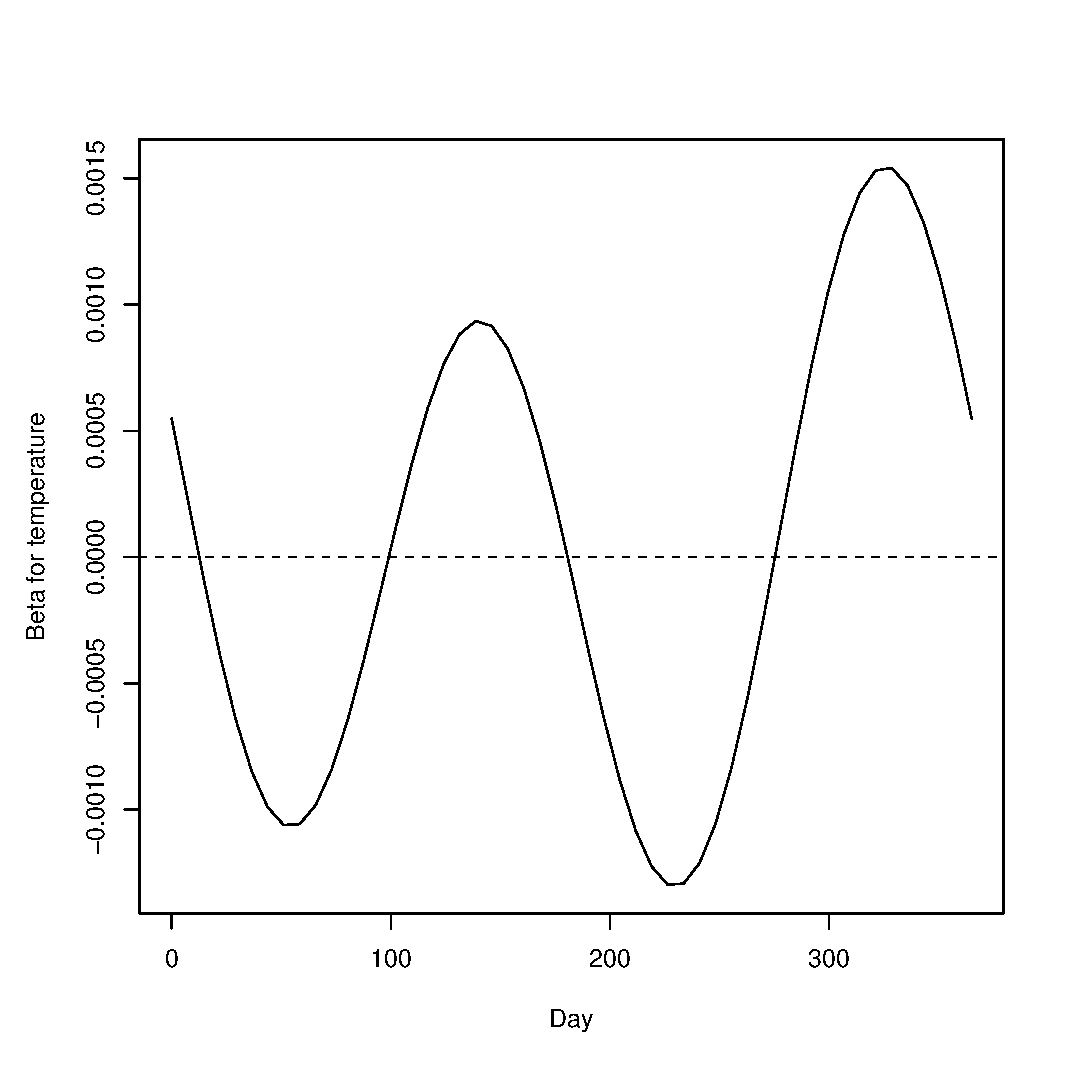
\includegraphics[height=7cm, width=11cm]{figs/precbeta5}
\newline \newline \newline
Ramsay, Hooker and Graves (2009)
\emph{Functional Data Analysis with R and Matlab}
(Springer, ch. 9)

\end{frame}

%%%%%%%%%%%%%%% fRegress.fdPar:  Concurrent Functional Model

\begin{frame}{fRegress.fdPar:  Concurrent Functional Model}

%\newline \newline \newline
Ramsay, Hooker and Graves (2009)
\emph{Functional Data Analysis with R and Matlab}
(Springer,ch. 10)

\end{frame}

%%%%%%%%%%%%%%% fRegress.formula:  Simple fRegress Setup

\begin{frame}{fRegress.formula:  Simple fRegress Setup}

\end{frame}

%%%%%%%%%%%%%%% linmod:  Full Integration Regression

\begin{frame}{linmod:  Full Integration Regression}

%\newline \newline \newline
Ramsay, Hooker and Graves (2009)
\emph{Functional Data Analysis with R and Matlab}
(Springer, ch. 10)

\end{frame}
%%%%%%%%%%%%%%% pda.fd:  Estimating a Differential Equation

\begin{frame}{pda.fd:  Estimating a Differential Equation}

%\newline \newline \newline
Ramsay, Hooker and Graves (2009)
\emph{Functional Data Analysis with R and Matlab}
(Springer, ch. 11)

\end{frame}
%%%%%%%%%%%%%%% Closing Remarks
\begin{frame}{Closing Remarks}

\end{frame}

%%%%%%%%%%%%%%% References
\begin{frame}{References}

%Software:   Ramsay, Wickham, Graves and Hooker (2009)
%\emph{fda: Functional Data Analysis. R package}, version 2.1.2
%(www.functionaldata.org)

%How to:  Ramsay, Hooker and Graves (2009)
%\emph{Functional Data Analysis with R and Matlab}
%(Springer, ch. 11)

%Theory:  Ramsay and Silverman (2005)
%\emph{Functional Data Analysis}, 2nd ed.
%(Springer)

\end{frame}

\end{document}
